\documentclass[main]{subfiles}
\begin{document}

%@@@@@@@@@@@@@@@@@@@@@@@@@@@@@@
% Main Topics: Neuromorphic 22.11.2018
% Lecturer: Giacomo Indiveri
% author: Vanessa Leite - base document from benelot/eth-intro-to-neuroinformatics-summary

\section{Neuromorphic VLSI}
\subsection{VLSI}
\begin{itemize}
	\item Very large scale integration technology allows to fabricate chips and memory.
	\item VLSI are usually digital, high power, not fault tolerant or robust, and clocked (synchronous), not massively parallel.
	\subitem The failure of one transistor is the failure of the computer
\end{itemize}

The computer hardware had a radical paradigm shift when we looked to real brains. For instance, a bee brain is much smaller and consume much less power (using neurons in a slow way), and offer real time interaction with the environment and complex behavior.

\subsubsection{Neuromorphic}
The term appeared in the 80's to describe VLSI systems containing electronic analog/digital circuits that exploit the physics of silicon to reproduce the bio-physics of neural circuits present in the nervous system.
\paragraph{Goals}
\begin{itemize}[noitemsep,nolistsep]
	\item Neuromorphic VLSI contain analog/digital circuits that exploit the physics of silicon to reproduce the bio-physics of neural circuits.
	\item The goals are to understand biological neural systems using standard CMOS VLSI technology as a tool.
	\item Known properties of biological systems can be exploited to design devices for engineering applications.
\end{itemize}

New hardware different of conventional computers: radically different from von Neumann architectures. Now, there are parallel elements with memory and computation co-localized, with continuous streaming data driven computation, no clock. The co-localization of memory and computation allows to have no I/O bottleneck and no memory bottleneck.

\paragraph{Neuromorphic computing vs engineering}
Neuromorphic computing uses a dedicated VLSI hardware, high performance computing, it is application driven and uses conservative approaches.
Neuromorphic engineering is a fundamental research, deeply rooted in biology. It emulates neural function in a subthreshold analog and asynchronous digital.

\subsection{Neuron circuits}
\begin{itemize}[noitemsep,nolistsep]
	\item Reproduce physics of neural computation using subthreshold analog circuits and asynchronous digital circuits.
	\item Build autonomous learning behaving systems that can interact with the environment in real-time.
	\item Best exploit for current and future VLSI technologies.
	\item Suited for nano and emerging technologies.
	\item Ideal tools for real- and accelrated-time modeling of neural systems.
	\item Compact, low-power sensory processing devices.
	\item Can interface directly with living systems.
\end{itemize}

\subsection{Circuits}
Digital transistors operating only in the minimum and the maximum. Analog transistor use also intermediate amounts, thus transistors can emulate physical proteic channels. In biology, at high voltages, the fraction of the channels that are open approaches unity, causing a saturation. The same can be seen in a subthreshold regime.
In subthreshold, the current is smaller than 1V, it increases exponentially, and after threshold currents changes quadratically. It changes from pico to nano amps.

\begin{figure}[H]
	\centering
	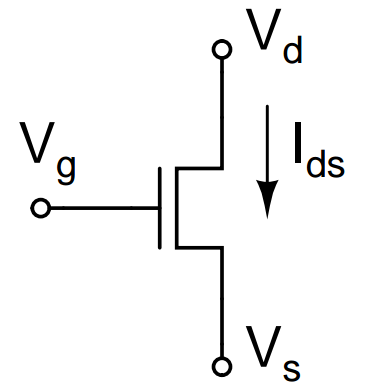
\includegraphics[width=0.2\textwidth]{mosfet.png}
\end{figure}

In Complementary Metal-Oxide Semiconductor (CMOS) technology, there are two types of MOSFETs: n-FETs and p-FETs. There is no current going to transistors.

In traditional CMOS circuits, all n-FETs have the common bulk potential $V_b$ connected to ground (GND) and all p-FETs have a common bulk potential connected to the power supply rail ($V_{dd}$).

\subsubsection{n-Fet subthreshold}
\begin{itemize}[noitemsep,nolistsep]
	\item $I_0$ current-scaling parameter.
	\item $\kappa_n$ subthreshold slope factor.
	\item $U_T$ the thermal voltage.
	\item $V_g$ the gate voltage, $V_s$ the source voltage, $V_d$ the drain voltage.
	\item The current is defined to be positive if it flows from the drain to the source.
	\item $I_{ds} = I_0e^{\kappa_n\frac{V_g}{U_T}}(e^{-\frac{V_s}{U_T}}-e^{-\frac{V_d}{U_T}})$
	\subitem $I_{ds} = I_0 e^{\kappa \frac{V_g}{U_T} - \frac{V_s}{U_T}} - I_0 e^{\kappa \frac{V_g}{U_T} - \frac{V_d}{U_T}} \rightarrow I_{ds} = I_f - I_r$.
	\item If $V_{ds} > 4U_T$ it becomes $I_{ds} = I_0e^{\kappa_n \frac{V_g}{U_T}-\frac{V_s}{U_T}}$
\end{itemize}

\subsubsection{p-Fet subthreshold}
The corresponding (complementary) equation for the p-FET:
\[ I_{ds}=I_0e^{\kappa_p(\frac{V_{dd}-V_g}{U_T})}(e^{-(\frac{V_{dd}-V_s}{U_T})}-e^{-(\frac{V_{dd}-V_d}{U_T})}) \]

\subsubsection{Differential-pair}
\begin{figure}[H]
	\centering
	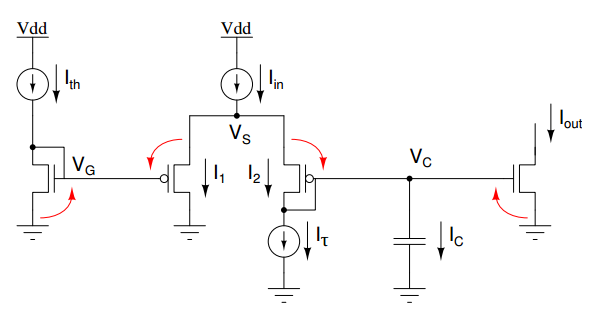
\includegraphics[width=0.5\textwidth]{dpi.png}
\end{figure}

\begin{itemize}
	\item $I_{in}=I_1+I_2$
	\item $I_2 = I_\tau + I_C$
	\item $I_{out} I_0 e^{\frac{kappa V_C}{U_T}}$
	\item $I_C = C\frac{d}{dt}V_C$
	\item $I_C = C \frac{U_T}{\kappa I_{out}} \frac{d}{dt}I_{out}$
	\item $\tau = \frac{CU_T}{\kappa I_\tau}$
	\item $I_{th} \cdot  I_1 = I_2 \cdot O_{out}$
	\item $I_{th} \cdot (I_{in} - I_\tau - I_C) = (I_\tau - I_C) \cdot I_{out}$
\end{itemize}

\[\tau(1 + \frac{I_{th}}{I_{out}}) \frac{d}{dt} I_{out} + I_{out}= \frac{I_{th} I_{in}}{I_\tau} - I_{th}\]

If $I_{in} >> I_{\tau}$:

\[\tau \frac{d}{dt} I_{out} + I_{out} = \frac{I_{th}}{I_\tau} I_{in}\]

For synapses:

\[\tau \frac{d}{dt} I_{syn} + I_{syn} = \frac{I_{th}}{I_\tau} I_{w}\]

\paragraph{Differential pair circuit}
\begin{itemize}
	\item $I_b = I_1 + I_2 = I_0 e^{\kappa \frac{V_b}{U_T}}$
	\item $I_1=I_b\frac{e^{\kappa \frac{V_1}{U_T}}}{e^{\kappa \frac{V_1}{U_T}}+e^{\kappa \frac{V_2}{U_T}}}$
	\item $I_2=I_b\frac{e^{\kappa \frac{V_2}{U_T}}}{e^{\kappa \frac{V_1}{U_T}}+e^{\kappa \frac{V_2}{U_T}}}$
\end{itemize}

The output currents of the diff-pair can be rewritten in the canonical sigmoid
form:
\[I_1=I_b\frac{1}{1 + e^{\frac{\kappa}{U_T} (V_2 - V_1)}}\]
\[I_2=I_b\frac{1}{1 + e^{\frac{\kappa}{U_T} (V_1 - V_2)}}\]

Difference of diff-pair currents:

\[I_1 - I_2 = I_b \frac{e^{\frac{\kappa V_1}{U_T}} - e^{\frac{\kappa V_2}{U_T}}}{e^{\frac{\kappa V_1}{U_T}} + e^{\frac{\kappa V_2}{U_T}}} = I_b \tanh(\frac{\kappa}{2U_T}(V_1 - V_2))\]


Two ways to implement the difference of currents: using a current mirror or a transconductance amplifier.

\paragraph{Current Mirror}
\begin{itemize}[noitemsep,nolistsep]
	\item Two MOSFETs of the same size.
	\item $I_{out}=e^{(V_{s1}-V_{s2})/U_T}I_{in}$
\end{itemize}

\paragraph{Transconductance Amplifier}
\[I_{out}=I_b\tanh(\frac{\kappa}{2U_T}(V_1-V_2))\]

For small differential voltages (e.g. $|V_1 - V_2| < 200 mV $), the $\tanh(\cdot)$ relationship is approximately linear and:

\[I_{out} \approx g_m(V_1-V_2)\]

where $g_m = \frac{I_b \kappa}{2_UT}$.

\subsection{Remarkable circuits}
\begin{itemize}
	\item McCulloch and Pitts artificial neuron model (first).
	\item Mahowald and Douglas conductance-based silicon neuron, similar to real cortical neurons, Figure a in ~\ref{fig:circuits}.
	\subitem properties remarkably similar to those of real cortical neurons
	\item Two main classes of neuron models: Conductance based, and Integrate and fire model (I\&F).
	\item Recently, Generalized Integrate and Fire models bridge the gap between the two.
\end{itemize}

\begin{figure}[H]
	\label{fig:circuits}
	\centering
	\begin{subfigure}[b]{0.5\textwidth}
		\centering
		\includegraphics[width=\textwidth]{conductance-based-SI-neuron.png}
		\caption{Conductance-based silicon neuron}
	\end{subfigure}%
	~
	\begin{subfigure}[b]{0.5\textwidth}
		\centering
		\includegraphics[width=\textwidth]{axon-hillock-circuit.png}
		\caption{Axon-Hillock-circuit}
	\end{subfigure}
\end{figure}
\begin{figure}[H]
	\centering
	\begin{subfigure}[b]{0.5\textwidth}
		\centering
		\includegraphics[width=\textwidth]{IanF-circuit.png}
		\caption{Ultra low-power generalized I\&F circuit}
	\end{subfigure}%
	~
	\begin{subfigure}[b]{0.5\textwidth}
		\centering
		\includegraphics[width=\textwidth]{multineuron-circuit.png}
		\caption{Spiking multineuron architectures}
	\end{subfigure}
\end{figure}

\subsection{Spikes and Adress Event Representation}

Adress Event Representation (AER) represents when a spike (action potential) arrives. At the time of a spike, the adress where the spike occurred is broadcast.

\subsection{Neuromorphic chips}
\subsubsection{Dynap: DYNamic neuromorphic Asynchronous Processor}
\begin{itemize}
	\item analog and digital co-design
	\item Distributed SRAM and TCAM memory cells
	\item On-chip inference and learning
\end{itemize}
\subsubsection{ROLLS: a Reconfigurable On-Line Learning Spiking chip}
\begin{itemize}
\item short-term plasticity
\item long-term plasticity
\item homeostatic plasticity
\item configurable recurrent connectivity
\end{itemize}

Many more...

\subsubsection{Neuromorphic Cognitive Systems}
\begin{itemize}
\item Working memory and decision making in autonomous real-time systems
\item Context dependent embedded systems and emerging technologies
\item Brain machine interfaces and prosthetics
\end{itemize}



\end{document}
